\chapter{Design and implementation}

\section{Initial design}	
The initial design for the game was an outcome of a few suggestions:
\begin{itemize}
\item the armband can best track the movement similar to natural movement of a forearm and do not translate so well to 2D movement (e.g. mouse control).
\item it is important to have cognitive elements that can translate to everyday life, like color recognition, using familiar objects.
\item the game focus should be on hand-eye coordination, so as a natural consequence, the idea of something appearing and the need to catch it/shoot it emerged. 
\end{itemize}
Based on that, I came up with an idea of \emph{The Battle of Rainbow Bridge}, shown in figure \ref{fig:design}. In the game, the player is a wizard, that has a magical wand. A lot of monsters appear in the sky and try to fly next to him to attack the city behind and he needs to stop them all. There are different type of monster and he need to use different spells to be able to destroy them. In a game, the player gradually learn new spells, one per each level. The movement of a wand is similar to movement of an forearm with elbow resting on the desk. 

\begin{figure}
\includegraphics[width=\textwidth]{graphics/described_drawing.png} 
\caption{The early concept of a game view. Number one is the wand, number two - the laser, number three - the monsters.}
\label{fig:design}
\end{figure}

The initial design is simple and not too detailed, because I have chosen to use Agile development method. I quickly built a prototype based on described design and tested it with children and adults. It allowed to receive continuous feedback and made game more entertaining and playable.

\subsection{Dictionary and mechanics}
\begin{itemize}
\item \emph{Asteroid} - check: \emph{Monster}
\item \emph{Failures} - counter for failed attempts in destroying \emph{Monsters}. Do not impact the game. 
\item \emph{Gate} - an object from which the \emph{Monsters} come from. It has a circle shape and is rotating counter-clockwise. There are 15 gates in the game, three rows with 5 each.
\item \emph{Laser} - a long object shot from the \emph{Wand} using gesture, able to destroy the \emph{Monster} if it has the same colour as it.
\item \emph{Level} - the game contains 5 levels, each one unlocking new gesture, so in first level player can only use one of them and on last one - all five. Each level is started with zero \emph{Successes} and \emph{Failures}.
\item \emph{Monster} - a rock-like, rotating object that is created in one of the \emph{Gates} and will stay, slowly growing. It will be destroyed if shot by a player with \emph{Laser} or after certain amount of time passes. If former, it counts as \emph{Success}, if latter, counts as \emph{Failure}. 
\item \emph{Successes} - counter for successfully destroyed \emph{Monsters}. If reaches appropriate number, player advance to next \emph{Level}
\item \emph{Wand} - an object, that can be wave around by the player. When player uses different gestures, \emph{Wand} can shoot with different coloured \emph{Lasers}. 
\end{itemize}

\section{Iterative testing}
\subsection{Testing of alpha version}

\textbf{State of the game:} The game supports controlling with one Myo device. It allows to shoot different colours lasers with different gestures. All asteroids are the same and they response to any kind of color. Backgrounds is an image. Basic UI counts successes and informs about Myo status (synchronized, connected etc.). Game is buggy, has stack overflow problems and allows accumulating not-destroyed asteroids in player's scene view.
\\
\textbf{Testing group:} three male adults, under 30 yo, with the supervision of author
\\
\textbf{Testing feedback:} 
\begin{itemize}
\item background and ground should be 3D structures to allow better depth recognition
\item the scene should have better lights
\item making the controls more advanced may result in more interesting game
\item missiles should be faster
\item using two hands for controlling seems to be interesting idea
\end{itemize}


\textbf{Design decisions:}
\begin{itemize}
\item background should be substituted with a skybox and a terrain with proper lightening 
\item the velocity of missiles should be increased
\item one hand should be now responsible for gestures and one for steering
\end{itemize}
\begin{figure}
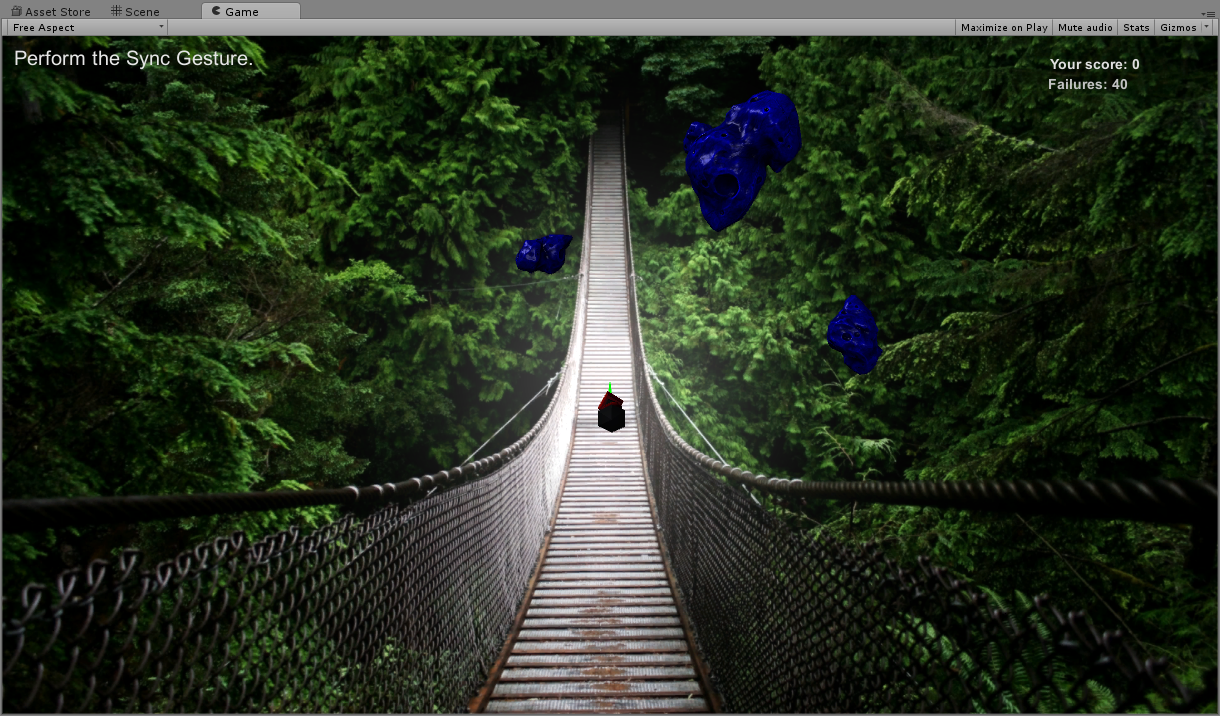
\includegraphics[width=\textwidth]{graphics/screen_v1.png} 
\caption{The alpha version of the game.}
\end{figure}

\subsection{Testing of beta version(children)}

\textbf{State of the game:} The game support controlling with two Myo devices - one for waving the wand and one for casting the spells with gestures. Lasers have better contrast. Asteroids have different colors and reacts only to lasers of appropriate colors. Background is now 3D terrain with skybox. The aim device has been introduced (green sight that gets red if on line with any target). The UI shows available gestures and their colors. Not destroyed asteroids now explode in front of the player. Objects like lasers and asteroids have time-based destructors to avoid the stack overflow. Levelling up mechanism has been implemented.
\\
\textbf{Testing group:} two girls, 9 years old and one adult, without supervision
\\
\textbf{Testing feedback:}
\begin{itemize}
\item aiming mechanism still too hard
\item two hands-based control works fine and even allows cooperative play
\item there are problem with calibrating the device and detecting the gestures
\end{itemize}


\textbf{Design decisions:}
\begin{itemize}
\item the aiming mechanism should be changed to whack-a-mole - monsters should appeared at predefines places on the 2D plane and do not move.
\end{itemize}
\begin{figure}
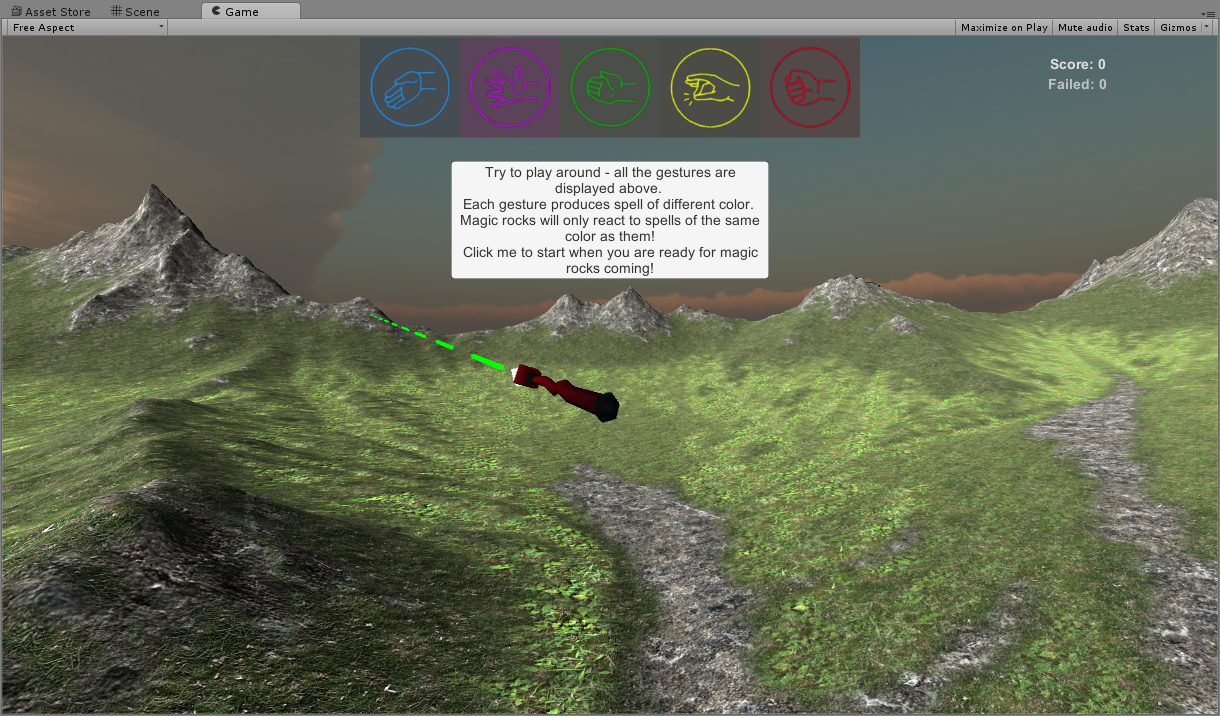
\includegraphics[width=\textwidth]{graphics/screen_v2a.png} 
\caption{The beta version of the game - training screen.}
\end{figure}

\begin{figure}
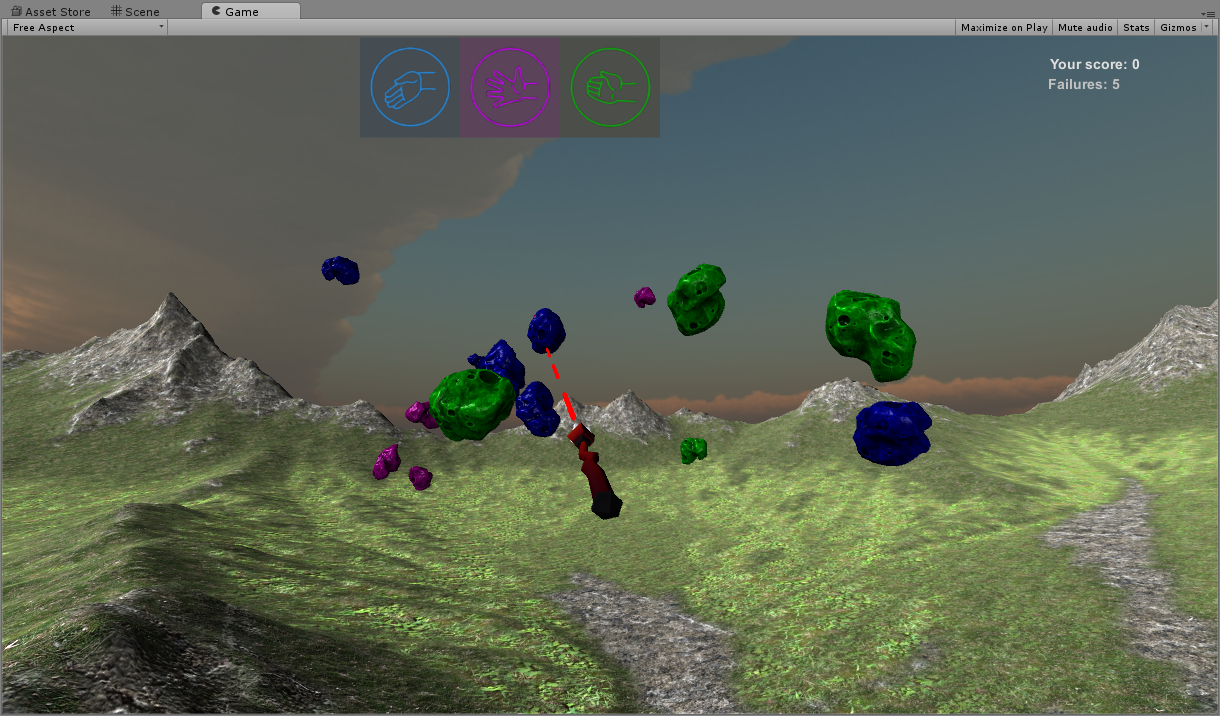
\includegraphics[width=\textwidth]{graphics/screen_v2b.png} 
\caption{The beta version of the game - casual screen view on third level.}
\end{figure}

\subsection{Testing of beta version(adults)}

\textbf{State of the game:} Same as in version for children.
\\
\textbf{Testing group}: 2 males, under 30 yo, with supervision of author
\\
\textbf{Testing feedback:}
\begin{itemize}
\item aiming problem persists
\item some gestures are not recognized as easily as the others
\item game was easily completed in a few minutes
\end{itemize}



\textbf{Design decisions}:
\begin{itemize}
\item same as in children testing
\end{itemize}

\subsection[Testing of version 1.0 (in debug mode)]{Testing of version 1.0 (in debug mode \footnote{Debug mode is run inside Unity instance and is significantly slower then Release Mode})}

\textbf{State of the game:} The "gate" concept was invent - now the screen contains 15 gates, that are spawning monsters. Monsters are spawned in the center of the gate and grow in size for some amount of time and disappear, if not destroyed. Single monster is never bigger than a gate. The statistic tool was added, counting how many and of what kind monsters were killed on each level. At the beginning of the game, game requires name, age and trial number, which it uses for creating a file with statistics. Number of spawned minions per level and time differences in spawning had been individualized per level. This version works by default with 2 Myos. This version includes sounds and music.
\\
\textbf{Testing group}: 1 boy (9yo), 1 male adult
\\
\textbf{Testing feedback}:
\begin{itemize}
\item there is problem with centering the wand
\item too many asteroids appear on the screen
\item second hand (steering hand) does not require to be synchronized
\item asteroids live too short
\end{itemize}


\textbf{Design decisions:}
\begin{itemize}
\item adjust number of asteroids appearing in final levels
\end{itemize}


\begin{figure}
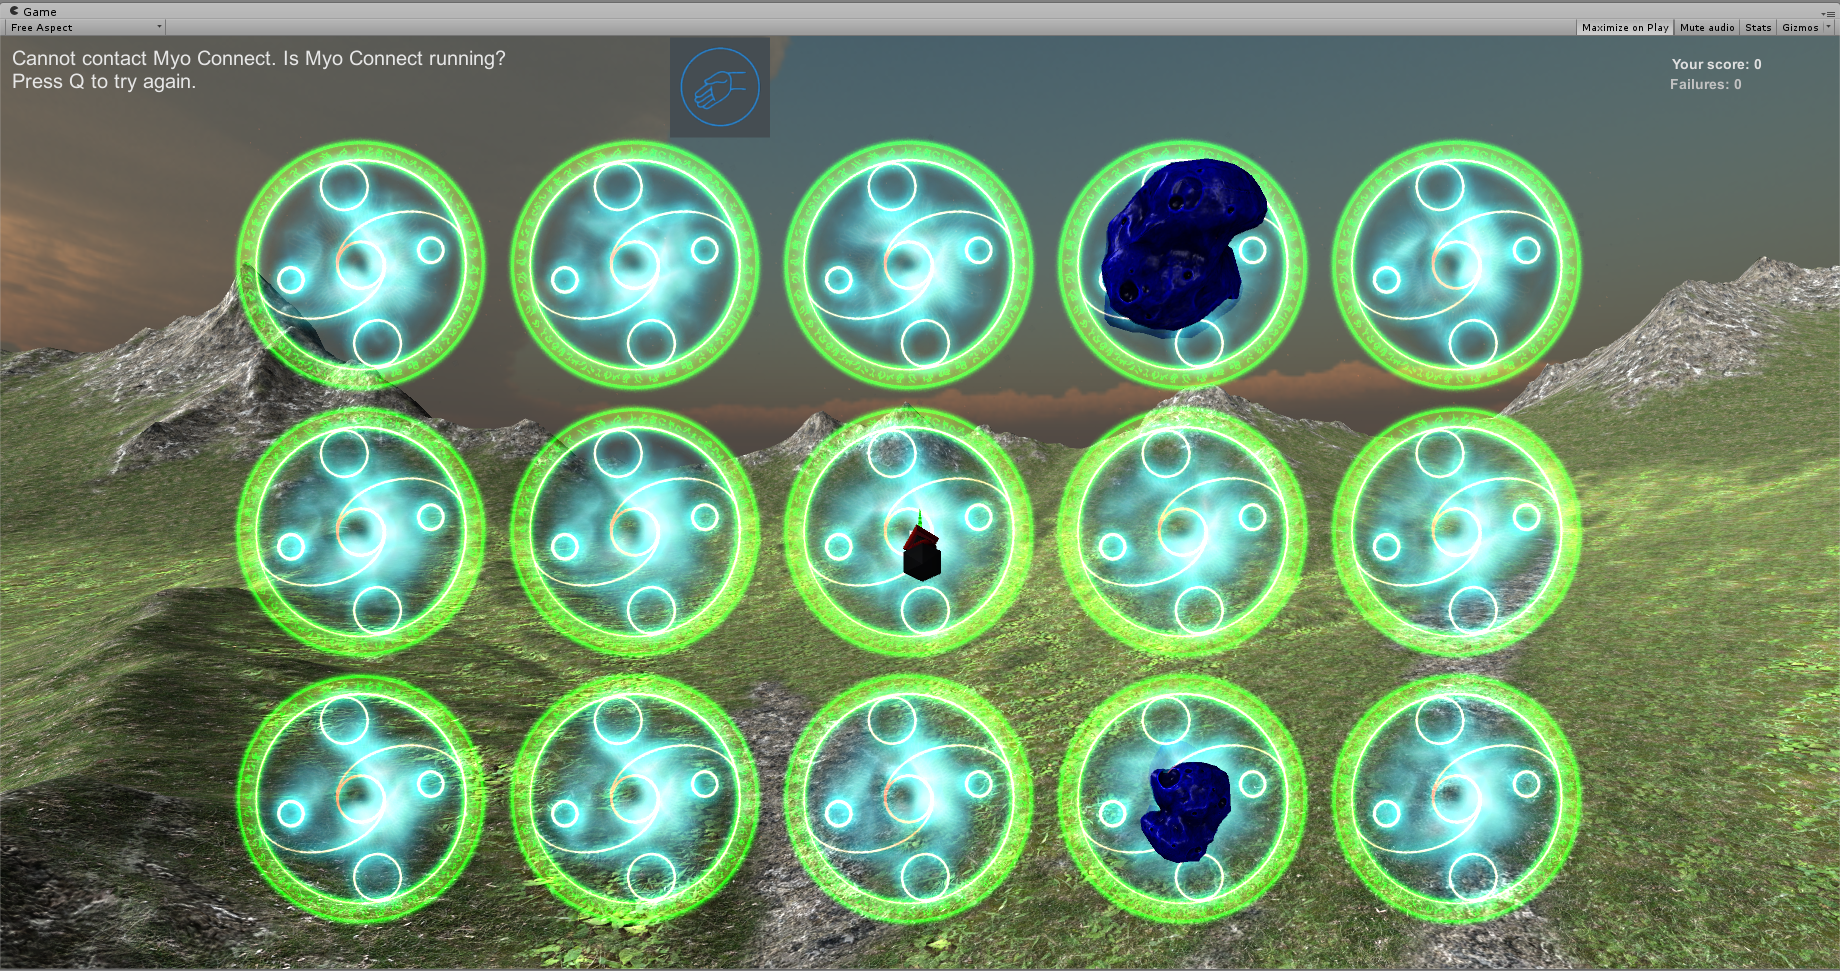
\includegraphics[width=\textwidth]{graphics/screen_v3.png} 
\caption{Version 1.0. The gates are spawning monsters, that are staying at the same place and only growing in size for defined amount of time before disappearing.}
\end{figure}

\subsection[Testing of version 1.0.1 (in debug mode)]{Testing of version 1.0.1 (in debug mode \footnotemark[\value{footnote}])}

\textbf{State of the game}: The number of asteroids for all levels has been adjusted (lowered).
\\
\textbf{Testing group}: 4 girls (6,8,10,11 yo), 1 male adult
\\
\textbf{Testing feedback}:
\begin{itemize}
\item the armband may require additional support (a band) for better fitting smaller arms 
\item asteroids seems to have appropriate or too short, depending on subject, length of life
\item sometimes it is not easy to remember appropriate gesture for appropriate color
\item the keyboard-based recentering does not seem to be natural
\item some subject has perceived wand movements not natural
\item the 6 yo was the only one whom hand was too small to detect the gestures
\end{itemize}


\textbf{Design decisions}:
\begin{itemize}
\item put recentering mechanism as a gesture of steering hand
\item display small information on asteroid about which gesture to use
\end{itemize}

\section{Design process}

\section{Implementation details}
